\chapter{Diagramas de clases UML}\label{apendice:a}
En la sección \ref{subsection:umlclases}, página \pageref{subsection:umlclases} se mostró el siguiente diagrama UML con elementos omitidos, ahora se presentarán el resto de diagramas completos.

\begin{figure*}[h]
	\begin{tikzpicture}
	
	\umlsimpleclass[y=-2.5]{MySemaforo}
	\umlsimpleclass[x=-6.6, y=0]{FuzzySet}
	\umlsimpleclass[x=6.5, y=-2.5]{MySensor}
	\umlsimpleclass[type=abstract]{FuzzySemaforo}
	
	\umlsimpleclass[x=-4, y=3.5]{TriangularMF}
	\umlsimpleclass[x=0, y=3.5]{SigmoidalMF}
	\umlsimpleclass[x=4, y=3.5]{GaussianaMF}
	
	\umlsimpleclass[x=-6.6, y=7]{FuzzyValue}
	\umlsimpleclass[x=0, y=7, type=abstract]{MembershipFunction}
	\umlsimpleclass[x=6.5, y=7, type=abstract]{SensorVehiculos}
	
	\umlunicompo[geometry=|-|, anchor1=140, mult1=1, mult2=0..*, pos2=2.8]{FuzzySemaforo}{TriangularMF}
	\umlunicompo[geometry=|-|, anchor1=90, mult1=1, mult2=0..*, pos2=2.8]{FuzzySemaforo}{SigmoidalMF}
	\umlunicompo[geometry=|-|, anchor1=40, mult1=1, mult2=0..*, pos2=2.8]{FuzzySemaforo}{GaussianaMF}
	
	\umlunicompo[mult1=1, pos1=0, align1=right, mult2=0..*, pos2=1, align2=left]{FuzzySemaforo}{FuzzySet}
	\umluniassoc[geometry=-|, anchor2=-130, attr2=cuenta vehículos|1, pos2=1, align2=right, align1=left, mult1=1, pos1=0]{FuzzySemaforo}{SensorVehiculos}
	\umlimpl[geometry=|-|]{TriangularMF}{MembershipFunction}
	\umlimpl[geometry=|-|]{SigmoidalMF}{MembershipFunction}
	\umlimpl[geometry=|-|]{GaussianaMF}{MembershipFunction}
	
	\umlimpl{MySensor}{SensorVehiculos}
	\umluniassoc[mult1=1, pos1=0, align1=right, mult2=0..1, pos2=1, align2=left]{MembershipFunction}{FuzzyValue}
	\umluniassoc[mult1=1, pos1=0.05, mult2=0..1, pos2=1, align2=left]{FuzzySet}{FuzzyValue}	
	
	\umlimpl{MySemaforo}{FuzzySemaforo}
	\end{tikzpicture}
	\caption{Diagrama de clases que muestra las relaciones del sistema}
	\label{uml:relaciones2}
\end{figure*}
\newpage

\section{Diagramas de las clases \textit{FuzzySet y FuzzyValue}}

\begin{figure}[H]
	\centering
	\begin{tikzpicture}
	
	\umlclass[anchor=north, y=-4]
	{FuzzySet}
	{- set\_u : vector< double > \\- set\_x : vector< double >}
	{+ FuzzySet( begin : double, step : double, end : double )\\
		+ FuzzySet( set : FuzzySet, f : MembershipFunction)\\
		+ operator>>( a : FuzzySet, b : FuzzySet) : FuzzySet\\
		+ operator\&( a : FuzzySet, b : FuzzySet) : FuzzySet\\
		%  	 + Print(show\_cero : bool ) : void \\
		+ get\_centroid() : double}
	
	\umlclass[]
	{FuzzyValue}
	{- x : double}
	{+ FuzzyValue( x : double) \\
		+ FuzzyValue( v : FuzzyValue)\\
		+ operator\_double() : double\\
		+ operator=( v : FuzzyValue) : FuzzyValue\\
		+ operator\&( v : FuzzyValue ) : FuzzyValue}
	\end{tikzpicture}
	\caption{Diagrama de las clases \emph{FuzzySet} y \emph{FuzzyValue}}
\end{figure}
\newpage

\section{Jerarquía de herencia \textit{MembershipFunction}}
El siguiente diagrama UML modela los miembros de las clases \textit{MembershipFunction, TriangularMF, SigmoidalMF, GaussianaMF}, además muestra su relación de herencia.


\begin{figure}[h]
	\centering
	\begin{tikzpicture}
	\umlclass[type=abstract]{MembershipFunction}{}{\umlvirt{+ operator()( x : double ) : FuzzyValue}}
	
	\umlclass[x=8.1, y=5]
	{TriangularMF}
	{- a : double\\- b : double\\- c : double}
	{+ TriangularMF( a : double, b : double, c : double )\\+ operator()( x : double ) : FuzzyValue }
	
	\umlclass[x=9, y=0]
	{SigmoidalMF}
	{- a : double\\- $x_0$ : double}
	{+ SigmoidalMF( a : double, $x_0$ : double )\\+ operator()( x : double ) : FuzzyValue }
	
	\umlclass[x=9, y=-5]
	{GaussianaMF}
	{- a : double\\- $x_0$ : double}
	{+ GaussianaMF( a : double, $x_0$ : double )\\+ operator()( x : double ) : FuzzyValue }
	
	\umlimpl[geometry=-|]{TriangularMF}{MembershipFunction}
	\umlimpl[]{SigmoidalMF}{MembershipFunction}
	\umlimpl[geometry=-|]{GaussianaMF}{MembershipFunction}
	\end{tikzpicture}
	\caption{Diagrama de clases que modela la jerarquía de herencia MembershipFunction }
\end{figure}


\newpage
\section{Realización de la clase \textit{SensorVehiculos}}
El siguiente diagrama modela los elementos omitidos de las clases \textit{SensorVehiculos} y \textit{MySensor}, además, se modela su relación de herencia y \emph{realización}.\\

\begin{figure}[h]
	\centering
	\begin{tikzpicture}
	\umlclass[type=abstract]
	{SensorVehiculos}
	{}
	{\umlvirt{+ read() : vector< double >} }
	
	\umlclass[y=-5]
	{MySensor}
	{ - num\_camaras : int }
	{ + SensorGenerico( camaras : int ) \\ + read() : vector< double > }
	
	\umlimpl[]{MySensor}{SensorVehiculos}
	
	\umlnote[x=-7, y=-5, anchor2=-160, width=4cm]{MySensor}{Esta clase es solo para demostración, deberá ser implementada adecuadamente por el usuario final }
	\end{tikzpicture}
	\caption{Diagrama de clases que modela la implementación de \textit{SensorVehiculos:read()}}
\end{figure}


\newpage
\section{Realización de la clase \textit{FuzzySemaforo}}
El siguiente diagrama modela los elementos omitidos de las clases \textit{FuzzySemaforo} y \textit{MySemaforo}, además, se modela su relación de herencia y \emph{realización}.\\

\begin{figure}[H]
	\centering
	\begin{tikzpicture}
	\umlclass[type=abstract]
	{FuzzySemaforo}
	{- num\_fases : int\\
		- num\_carriles : int\\
		- num\_avenidas : int\\
		- fase : int \\
		- tiempo : double\\
		- vehiculos : double\\
		- congestion : double\\
		- autos : vector< double >\\
		- pesos : vector< double >\\
		- ciclo : Ciclo\\
		- carriles : Carril\\
		- sensor : SensorVehiculos}
	{+ FuzzySemaforo( ciclo:Ciclo, carril:Carril, sensor:SensorVehiculos )\\
		+ run() : void\\
		\umlvirt{+ set\_lights( fase : int, tiempo : double ) : void}\\
		- get\_time( t : int, c : int) : double\\
		- get\_media( fase : int, estado : int)}	
	
	\umlclass[y=-9]{MySemaforo}{}
	{+ MySemaforo(ciclo:Ciclo, carriles:carril, sensor:SensorVehiculos)\\
		+ set\_lights( fase : int, tiempo : double) : void}
	
	\umlimpl{MySemaforo}{FuzzySemaforo}
	\umlnote[x=-8, y=-9, width=3cm]{MySemaforo}{Esta clase es solo para demostración, deberá ser implementada adecuadamente por el usuario final }
	\end{tikzpicture}
	\caption{Diagrama de clases que modela la implementación de \textit{set\_lights: FuzzySemaforo}}
\end{figure}
